\documentclass{article}

\usepackage{amssymb,amsmath}
\usepackage[utf8]{inputenc}
\usepackage{graphicx}
\usepackage[section]{placeins}
\usepackage[
bookmarks=true,
colorlinks=true,
breaklinks=true,
urlcolor=red,
citecolor=blue,
linkcolor=black,
unicode=true,
]
{hyperref}

\begin{document}
\section{SVM, Adaboost}
\subsection{Lineární SVM}
SVM je lineární klasifikátor minimalizující strukturální risk. SVM řeší kvadratickou optimalizační úlohu:

\begin{gather}
minimize \  \frac{1}{\|w\| ^2}\\
s.t.:\ y_i(w\cdot  x_i + b) \geq 1, i \in \{1, ..., N\} 
\end{gather}

Duální úloha: 

\begin{gather}
maximize \  L(\textbf{h}) = \displaystyle\sum_{i = 1}^N h_i - 0.5 \cdot \textbf{h} \cdot \textbf{D} \cdot \textbf{h}\\
s.t.:\ \textbf{h} \cdot \textbf{y} = 0\\
h \geq 0
\end{gather}
Kde \textbf{h} je vektor lagrangeových multiplikátorů a $D = y_i y_j x_i\cdot x_j$ ($x_i$ a $x_j$ jsou vektory, $D$ matice). Vektor \textbf{h} má nenulové prvky jenom pro support vectory.\\

Když nejsou data lineárně separovatelné dodáme slackové proměnné $\sigma$, které nám dovolí relaxovat problém zanedbáním některých pozorování. Formulace problému se změní následovně: 

\begin{gather}
minimize \  \displaystyle\frac{1}{\|w\| ^2} + C\sum_{i=1}^N\sigma_i \\
s.t.:\ y_i(w\cdot  x_i + b) \geq 1 - \sigma_i , i \in \{1, ..., N\}\\
\sigma_i \geq 0 , i \in \{1, ..., N\}
\end{gather}

a duální:

\begin{gather}
maximize \  L(\textbf{h}) = \displaystyle\sum_{i = 1}^N h_i - 0.5 \cdot \textbf{h} \cdot \textbf{D} \cdot \textbf{h}\\
s.t.:\ \textbf{h} \cdot \textbf{y} = 0\\
 0 \leq \textbf{h} \leq C
\end{gather}

Shrnutí v Figure \ref{fig:SVM_overview}.

\begin{figure}[h]
\begin{center}
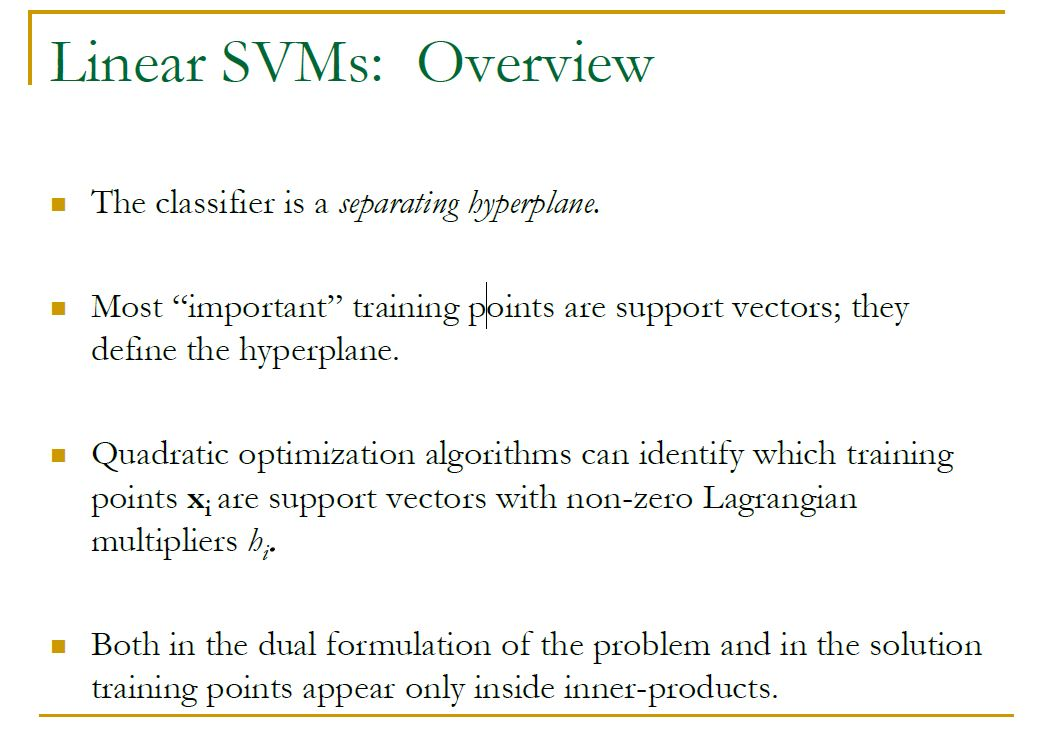
\includegraphics[width=12cm]{SVM_overview.jpg}
\caption{SVM shrnutí}
\label{fig:SVM_overview}
\end{center}
\end{figure}

\subsection{Nelineární SVM}

Základní myšlenka je že namapujeme originální, nadrovinou nerozdělitelná data do prostoru větší dimenze, kde už to půjde. Příklad ve Figure \ref{fig:SVM_example}. Pro tuto akci využijeme vlastnost, že SVM závisí pouze na skalárním součinu $x_i \cdot x_j$. Tento součin nahradíme jádrovou funkcí která bude mapovat naše data do prostoru s vyšší dimenzí. Příklady jádrových funkcí ve Figure \ref{fig:kernel_examples}. Celkové shrnutí SVM v \ref{fig:overall_summary}.
Formulace problému tentokrát už jenom v duálu: 

\begin{gather}
maximize \  L(\textbf{h}) = \displaystyle\sum_{i = 1}^N h_i - 0.5 \cdot \textbf{h} \cdot \textbf{D} \cdot \textbf{h}\\
s.t.:\ \textbf{h} \cdot \textbf{y} = 0\\
 0 \leq \textbf{h} \leq C\\
 \textbf{D} = y_i y_j K(\textbf{x}_i, \textbf{x}_j)
\end{gather}

\begin{figure}[h]
\begin{center}
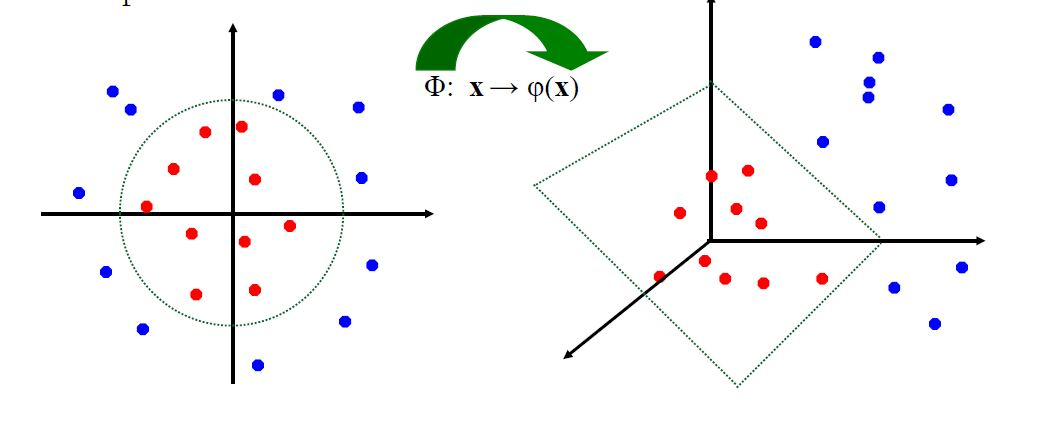
\includegraphics[width=12cm]{nonlinearSVM_example.jpg}
\caption{Nonlinear SVM example}
\label{fig:SVM_example}
\end{center}
\end{figure}

\begin{figure}[h]
\begin{center}
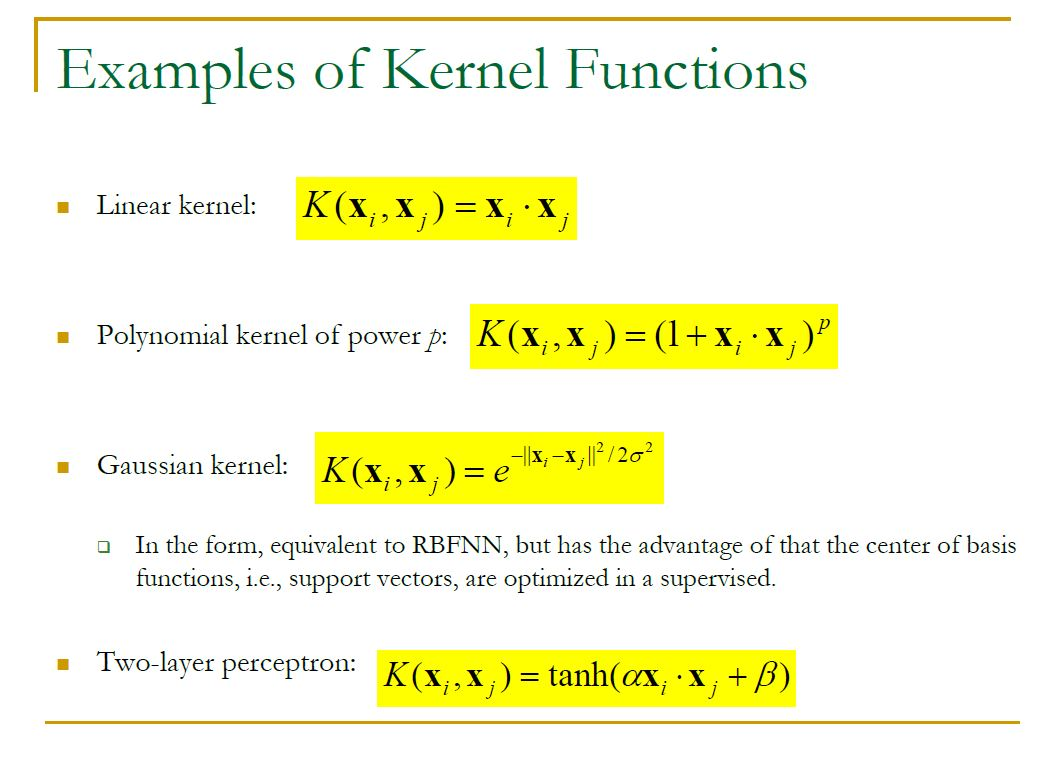
\includegraphics[width=12cm]{kernel_examples.jpg}
\caption{Jádrové funkce}
\label{fig:kernel_examples}
\end{center}
\end{figure}

\begin{figure}[h]
\begin{center}
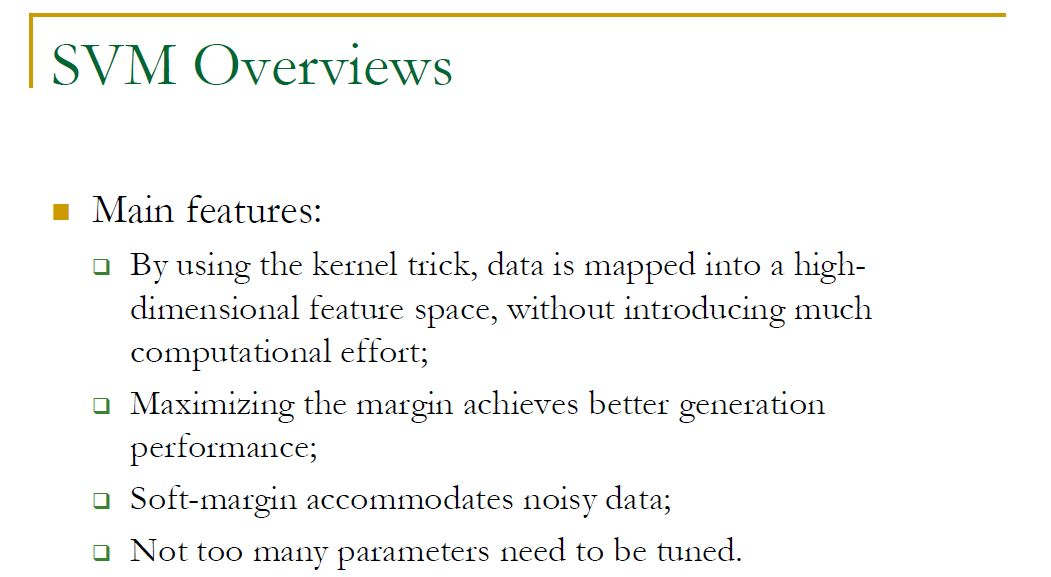
\includegraphics[width=12cm]{overall_summary.jpg}
\caption{Shrnutí SVM}
\label{fig:overall_summary}
\end{center}
\end{figure}

\section{Adaboost}
Úvod k algoritmu v \ref{fig:adaboost_itroduction}, popis algoritmu v Figure \ref{fig:adaboost_summary} a výhody a nevýhody v Figure \ref{fig:adaboost_pros_cons}.

\begin{figure}[h]
\begin{center}
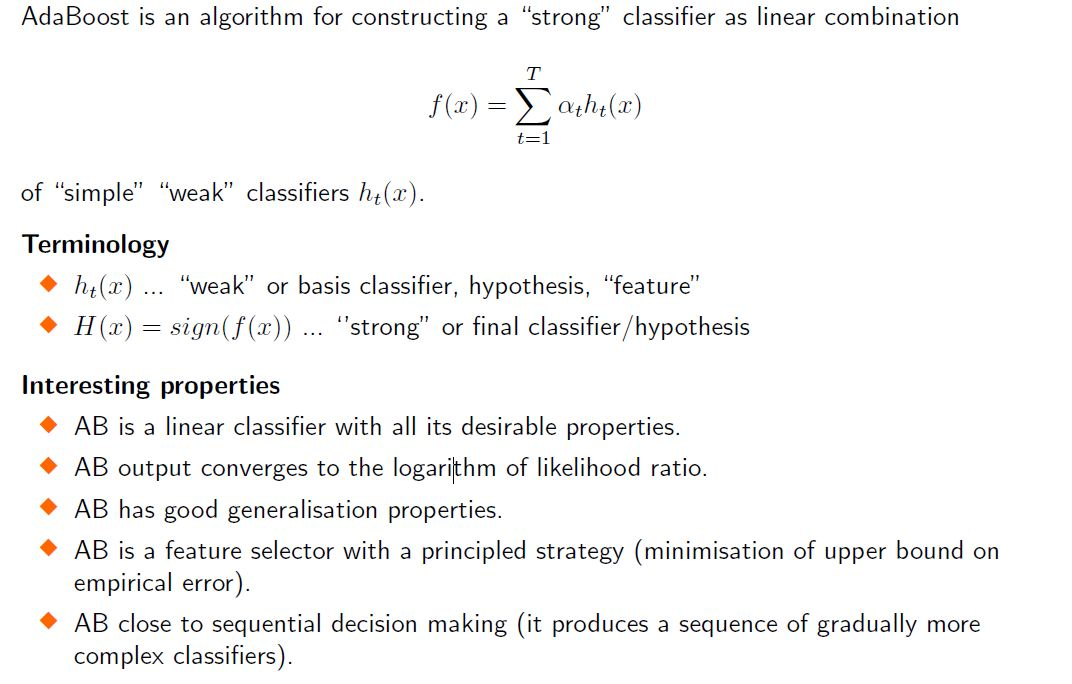
\includegraphics[width=12cm]{adaboost_introduction.jpg}
\caption{Úvod k adaboost}
\label{fig:adaboost_itroduction}
\end{center}
\end{figure}

\begin{figure}[h]
\begin{center}
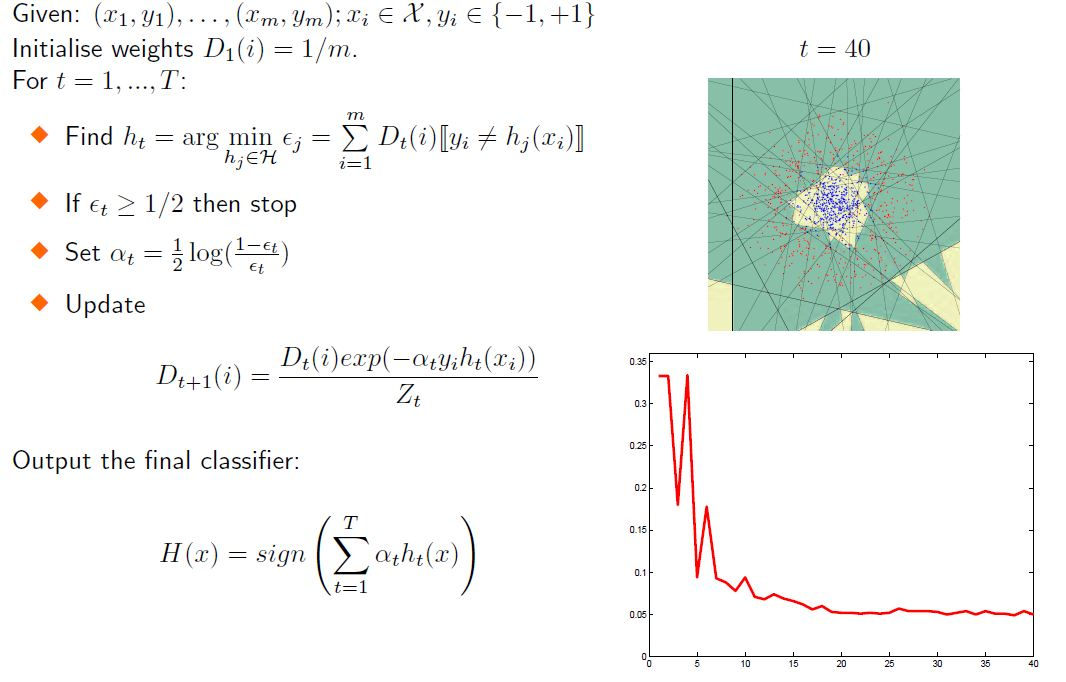
\includegraphics[width=12cm]{adaboost_summary.jpg}
\caption{Shrnutí adaboostu}
\label{fig:adaboost_summary}
\end{center}
\end{figure}

\begin{figure}[h]
\begin{center}
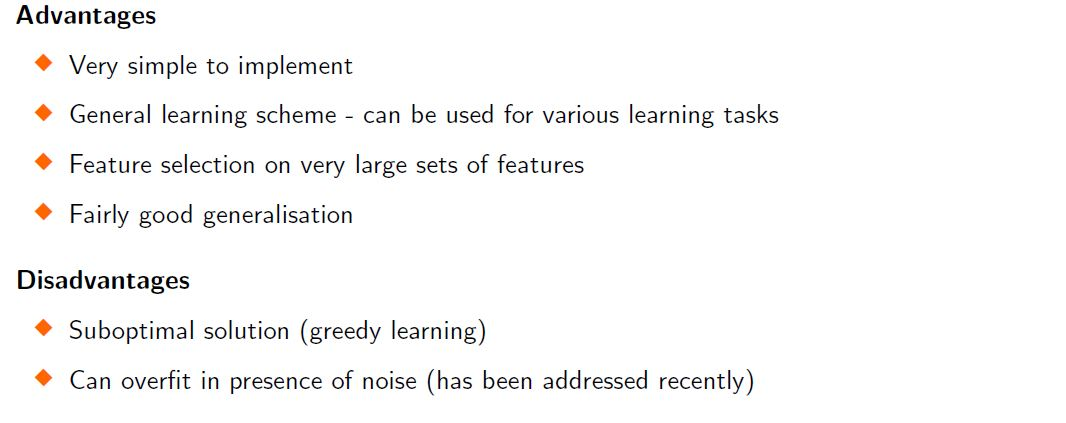
\includegraphics[width=12cm]{adaboost_pros_cons.jpg}
\caption{Výhody a nevýhody}
\label{fig:adaboost_pros_cons}
\end{center}
\end{figure}
\end{document}